\begin{figure}
\centering
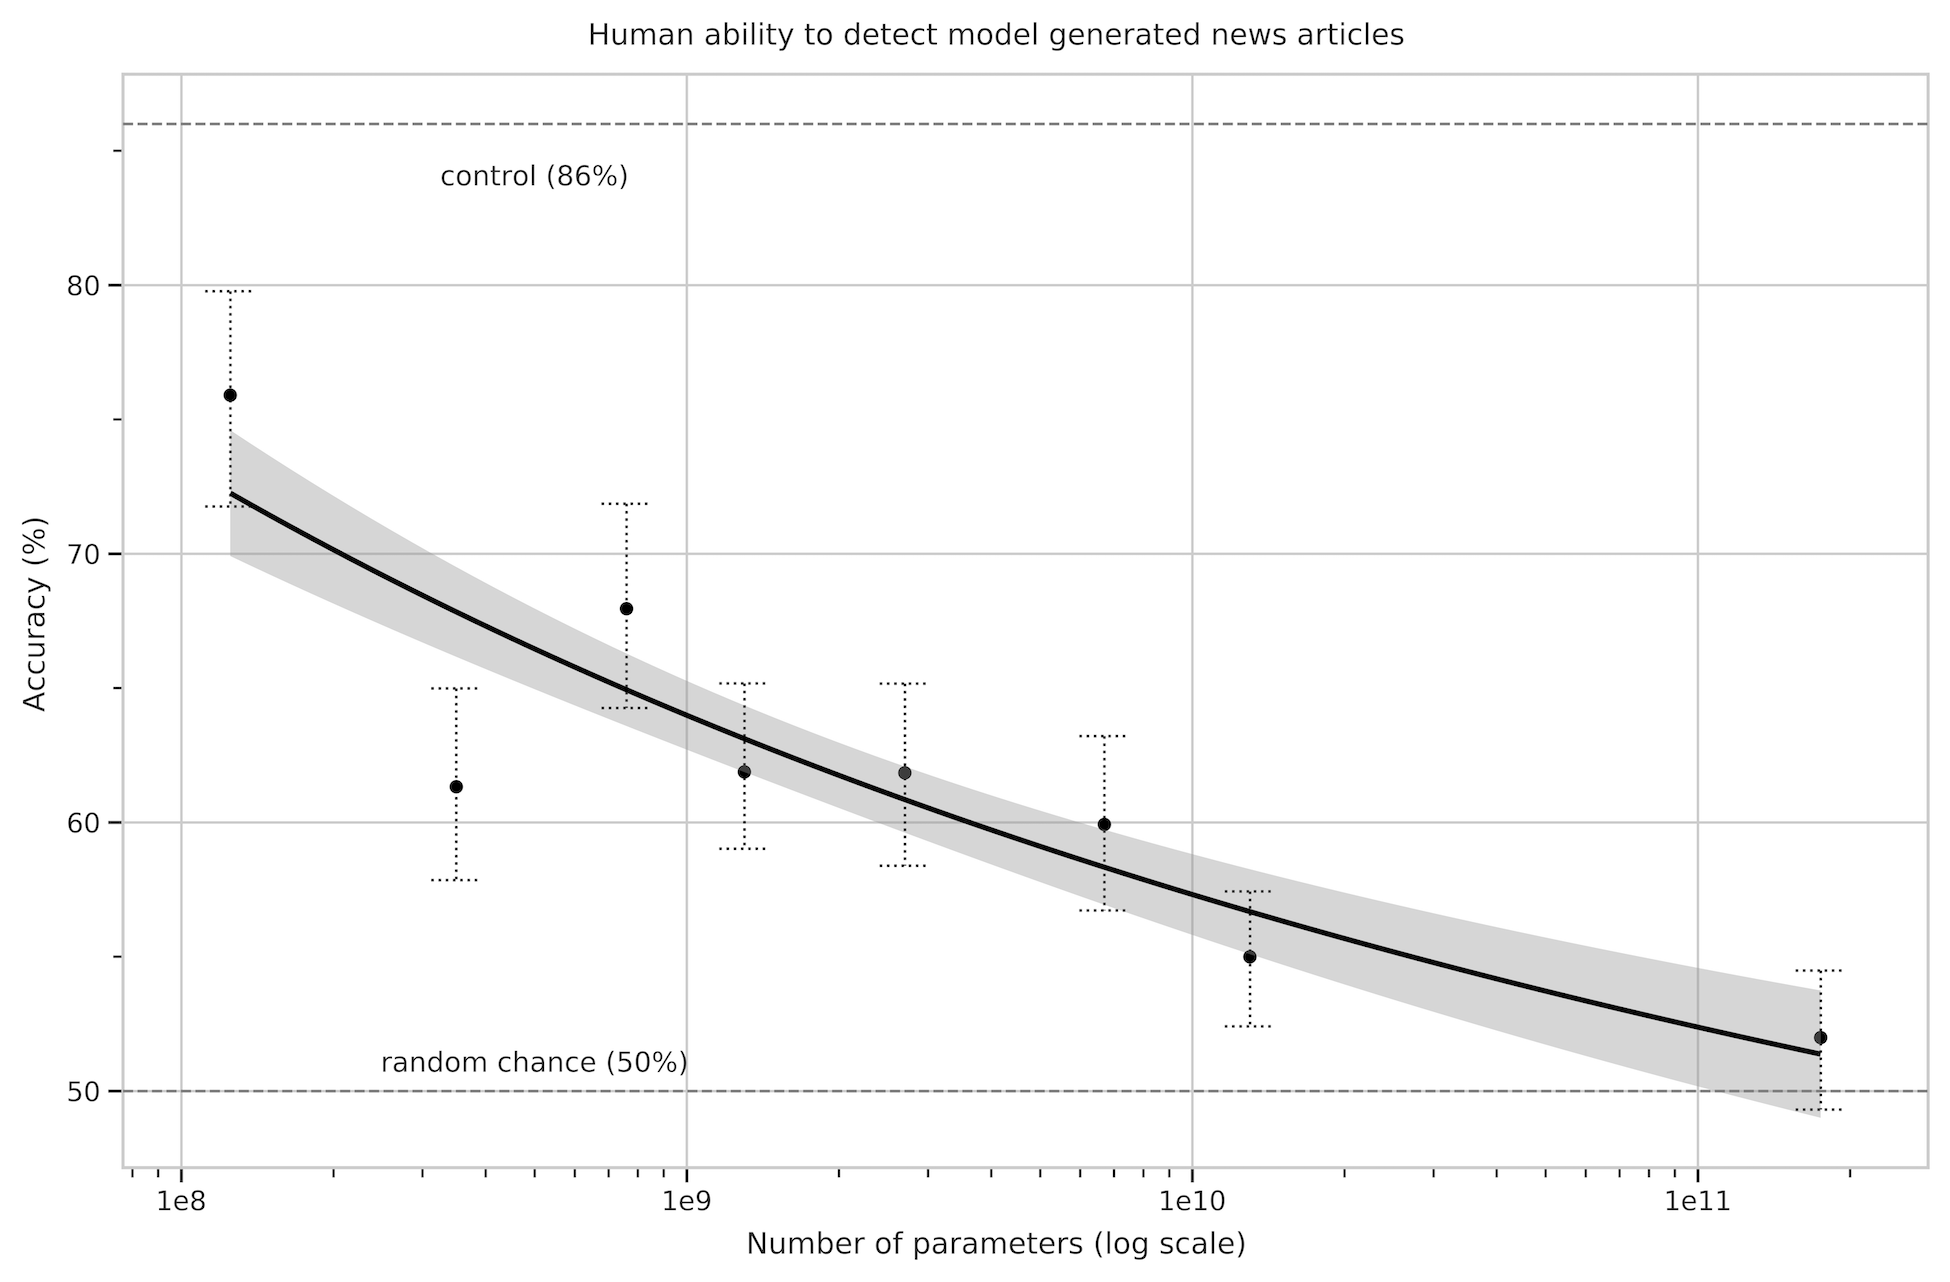
\includegraphics[width=\linewidth]{graphs/img/generation_plot.png}
\caption{People's ability to identify whether news articles are model-generated (measured by the ratio of correct assignments to non-neutral assignments) decreases as model size increases. Accuracy on the outputs on the deliberately-bad control model (an unconditioned GPT-3 Small model with higher output randomness) is indicated with the dashed line at the top, and the random chance (50\%) is indicated with the dashed line at the bottom. Line of best fit is a power law with 95\% confidence intervals.}
\label{graph:generation}
\end{figure}